\documentclass[UTF8,12pt]{exam}
\usepackage{ctex}
%使用中文包
\usepackage[paper=a4paper,margin=2cm]{geometry}
%使用A4纸张,2cm页边距
\usepackage{amssymb}%区别于amsmath宏包的高级版本
\usepackage{mathtools}%amsmath宏包的兼容版,升级版

\usepackage{tikz}%用于绘制图形,例如四棱锥
\usepackage{graphicx}
\pointpoints{}{} % 单数/复数形式均设为中文"分"



\DeclarePairedDelimiter{\paren}{(}{)} % 定义 \paren 自动匹配括号

%设置页面样式为headandfoot(由exam文档类提供),表示页眉和页脚都会显示。
\pagestyle{headandfoot}

%针对试卷的后续页脚给于一个详细的解释
\firstpageheader{2025年普通高等学校招生全国统一考试}{}{\bfseries\large 数学(新高考I卷)}
\firstpagefooter{}{\footnotesize 第\thepage\ 页(共\numpages\ 页)}{}
%针对试卷的后续页脚给于一个详细的解释
\runningheader{}{}{}
\runningfooter{}{\footnotesize 第\thepage\ 页(共\numpages\ 页)}{}

\title{2025年新高考数学I卷模拟试题}
\author{}
\date{ 2025年 6 月 7 日}

\begin{document}

\everymath{\displaystyle}
%设置行内数学公式默认使用\displaystyle(显示样式),这样行内公式也会以行间公式的大小显示,但可能会影响行距。
\maketitle

\begin{center}
\textbf{注意事项:}
\begin{enumerate}
  \item 答卷前,考生务必用黑色签字笔填写姓名和准考证号
  \item 选择题用2B铅笔填涂,非选择题用签字笔作答
  \item 考试时间120分钟,满分150分
\end{enumerate}
\end{center}

\section*{一、单选题(共8小题,每题5分,共40分)}
%\paren 由数学宏包(如 mathtools 或 physics)提供,用于生成自适应大小的数学括号(如 \left( %\right)),必须用在数学模式中13。
% 效果: x = \left( \frac{a}{b} + c \right)
%\hfill  <x-preset  class="no-tts  reference-tag disable-to-doc"  data-index="5">5</x-preset>
% 禁止文本转语音 引用标记  禁止导出到文档
\begin{questions}
\question 已知复数 $z=\dfrac{3-i}{1+2i}$,则 $|z|=  $ \hfill $\paren{ \ \ \ \ \   } $
%使用w文本模式中 \hfill 作用:创建弹性水平空间,将后续内容推到行尾
\begin{choices}
\choice $\sqrt{2}$  
\choice $\dfrac{\sqrt{10}}{2}$ 
\choice $\dfrac{3\sqrt{2}}{2}$ 
\choice $\sqrt{5}$
\end{choices}

\question 样本数据 $2, 8, 14, 16, 20$ 的平均数为 \hfill  $\paren{\ \ \ \ \ }$
\begin{choices}
\choice $8$
\choice $9$
\choice $12$
\choice $15$
\end{choices}

\question 已知集合 $A=\{x| \ln(x-1) < 0\}$, $B=\{x| x^2-3x<0\}$,则 $A\cap B=$ \hfill $\paren{\ \ \ \ \ \ \ }$
\begin{choices}
\choice $(1,2)$
\choice $(1,3)$
\choice $(0,3)$
\choice $(2,3)$
\end{choices}

\question 抛物线 $y^2=4x$ 的焦点为 $F$,点 $A$ 在抛物线上且 $|AF|=5$,则点 $A$ 到 $y$ 轴距离为  \hfill $\paren{\ \ \ \ \ \ \ }$
\begin{choices}
\choice $3$
\choice $4$
\choice $5$
\choice $6$
\end{choices}

\end{questions}
%与\frac相比,\dfrac这个命令强制分数以较大的形式显示
\section*{二、多选题(共3小题,每题6分,共18分)}
\begin{questions}
\question 已知函数 $f(x)=\sin\left(2x+\dfrac{\pi}{3}\right)$,则 \hfill $\paren{\ \ \ \ \ \ \ }$
\begin{checkboxes}
\choice $f(x)$ 周期为 $\pi$  
\choice $x=\dfrac{\pi}{12}$ 是函数对称轴
\choice $\left[-\dfrac{\pi}{3},0\right]$ 上单调递增
\choice 值域为 $[-1,\sqrt{3}]$
\end{checkboxes}

\question 在 $\triangle ABC$ 中,$\overrightarrow{AB}\cdot\overrightarrow{AC}=6$,$|\overrightarrow{AB}|=3$,$|\overrightarrow{AC}|=4$,则 \hfill $\paren{\ \ \ \ \ \ \ }$
\begin{checkboxes}
\choice $\angle BAC = 60^\circ$  
\choice $S_{\triangle ABC}=3\sqrt{3}$  
\choice $|\overrightarrow{BC}|=\sqrt{13}$ 
\choice $\overrightarrow{BA}$ 在 $\overrightarrow{BC}$ 投影为 $-\dfrac{9}{\sqrt{13}}$
\end{checkboxes}
\end{questions}

\section*{三、填空题(共3小题,每题5分,共15分)}
\begin{questions}
\question $\displaystyle\int_0^{\pi/2} \cos^3 x\, dx = $\underline{\hspace{2cm}} 

\question 三棱锥 $P-ABC$ 体积为 $12$,若点 $Q$ 满足 $\overrightarrow{PQ}=\dfrac{3}{4}\overrightarrow{PA}$,则四面体 $Q-ABC$ 体积为\underline{\hspace{2cm}} 

\question 已知数列 $\{a_n\}$ 满足 $a_1=1$,$a_{n+1}=\dfrac{2a_n}{a_n+3}$,则 $a_{2025}=$\underline{\hspace{2cm}} 
\end{questions}


%您使用的文档类(如 exam 或其他试题模板)默认使用英文术语(如 "points")标注分值。
%您在 \question 命令中显式指定了中文分值 [17分],但模板的分值标签生成机制仍自动附加了英文词 %"points"。


\section*{四、解答题(共5小题,共77分)}
\begin{questions}
%方括号 [] 内为可选参数,question是exam 的题目容器命令,用于包裹所有试题
\question [13分] 在 $\triangle ABC$ 中,$a,b,c$ 分别为角 $A,B,C$ 对边,且 $b\cos C + c\cos B = 2a\cos A$ 

\begin{parts}
\part 证明:$2\cos A = 1$
\part 若 $a=2$,$c-b=1$,求 $\triangle ABC$ 面积
\end{parts}

\question [15分] 如图,四棱锥 $P-ABCD$ 底面为正方形,$PD\perp$ 底面 $ABCD$,$PD=AD=2$
\begin{center}
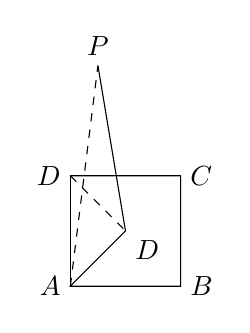
\begin{tikzpicture}[scale=0.7]
\draw (0,0)--(2,0)--(2,2)--(0,2)--cycle;
\draw (1,1) node[below right]{$D$}--(0,0) node[left]{$A$}--(2,0) node[right]{$B$}--(2,2) node[right]{$C$}--(0,2) node[left]{$D$};
\draw (1,1)--(0.5,4) node[above]{$P$};
\draw[dashed] (0,2)--(1,1) (0,0)--(0.5,4);
\end{tikzpicture}
\end{center}
\begin{parts}
\part 证明:$BD \perp PC$ %数学中的垂直命令
\part 求二面角 $A-PB-C$ 的正弦值
\part 在线段 $PB$ 上是否存在点 $M$ 使 $AM\parallel$ 平面 $PCD$?说明理由
\end{parts}

\question [15分] 已知函数 $f(x)=e^x - ax - \cos x$。
\begin{parts}
\part 当 $a=1$ 时,求 $f(x)$ 的极值点个数
\part 若 $f(x)\geq 0$ 恒成立,求整数 $a$ 的最大值
\end{parts}

\question [17分] 双曲线 $C:\dfrac{y^2}{4} - x^2 = 1$,过点 $P(0,3)$ 的直线 $l$ 交 $C$ 于 $M,N$ 两点.
\begin{parts}
\part 当 $l$ 斜率不存在时,求 $\triangle OMN$ 面积($O$ 为原点)
\part 记 $Q$ 为 $MN$ 中点,证明:$k_{OQ} \cdot k_l = \dfrac{1}{2}$
\part 是否存在 $l$ 使得 $\angle MON=90^\circ$?若存在求 $l$ 方程,否则说明理由
\end{parts}

\question [17分] 投掷一枚均匀硬币 $n$ 次,$X$ 表示正面向上次数.\hfill 
\begin{parts}
\part 求 $P(X=2k)$ 关于 $k$ 的表达式
\part 证明:$\displaystyle \sum_{k=0}^{\lfloor n/2 \rfloor} P(X=2k) = \dfrac{1}{2}$
\part 设 $Y=|X - \dfrac{n}{2}|$,求 $E(Y)$ 表达式
\end{parts}
\end{questions}

\begin{center}

\textbf{(试卷结束)}
\end{center}

\end{document}